\section{The Proxy module}

\subsection{Introduction}
\label{sec:proxy_introduction}

%~\cite{GoF}
The purpose of the Proxy module is to hide the internal architecture of the IPOL system and to provide a unique entry point for the communication between its different modules. It is technically a \emph{Reverse Proxy} \footnote{\url{https://en.wikipedia.org/wiki/Reverse_proxy}}.

The proxy solves several problems, as for example the strong dependency between the machines where the other modules are located. For instance, if we want to change the location of one of our IPOL modules, we only need to modify the information file used in the proxy. As a consequence, the system does not need more modifications. Figure ~\ref{fig:proxy_example} shows an example.

\begin{figure}[!ht]
\centering
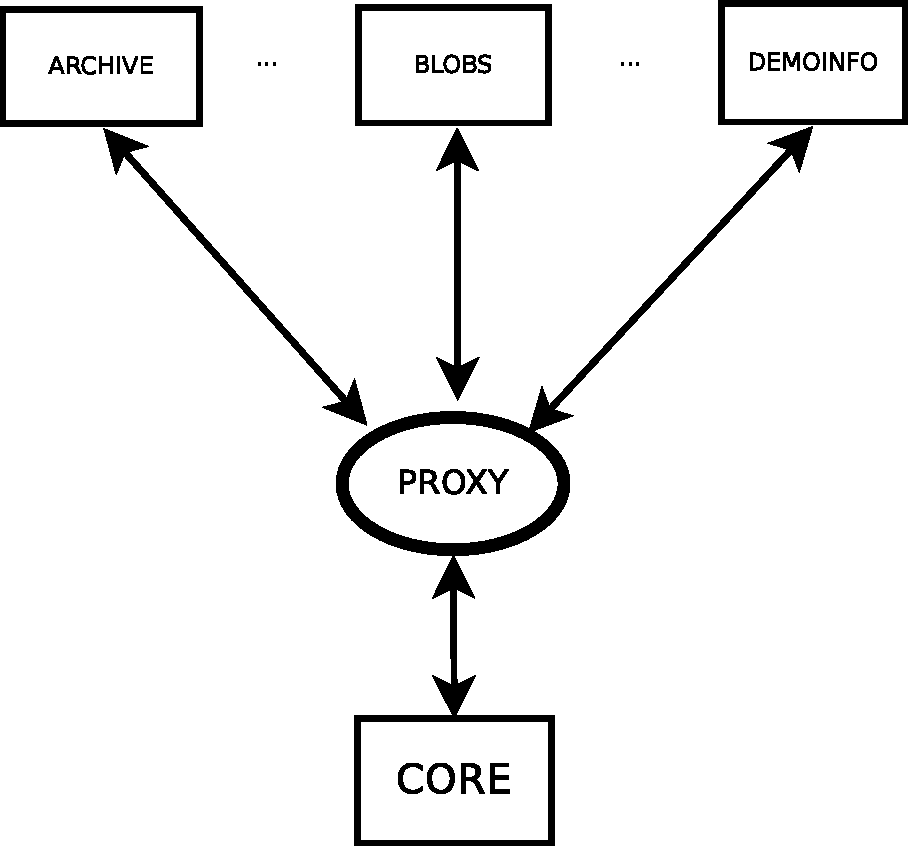
\includegraphics[width=0.5\columnwidth]{proxy/images/proxy_diagram.pdf}
\caption{The reverse proxy is the communication entry point to the system and hides its internal architecture.} 
\label{fig:proxy_example}
\end{figure}

\paragraph{Technologies used} \hspace{0pt} \\
The module is written in Python within the Cherrypy framework. The other modules must communicate with the proxy using a proper format in the URL (see Sec.~\ref{sec:request_format}) while the output is JSON encoded.

\subsection{Architecture}

\paragraph{Module composition} \hspace{0pt} \\
The module is composed of the following files: the code itself in: “proxy.py”, a main file for initiating the module: “main.py” and a cherrypy configuration file: “proxy.conf”. It also uses a log file where the modules registers error messages. The logs directory is specified at the ``proxy.conf” configuration file.

\paragraph{Module architecture} \hspace{0pt} \\

The module is encapsulates within a single class ’Proxy’. The services offered by the module are all methods of this class. The cherrypy framework provides the abstraction for making the methods available as services. In the case of the proxy, it only has two services: ping and shutdown.

The CherryPy engine is launched when the module starts. Besides, it loads the cherrypy configuration from “proxy.conf”. It also creates (if not exist) a logs folder using the information from the cherrypy configuration file and stores all the modules information provided by the XML file as a dictionary.

When other module requests a service, it must communicate with the proxy using arguments given through an URL. The latter must follow a few guidelines. If the requesting module does not fulfill with the required specifications, the proxy returns a JSON message that notifies the error and writes it in the file “error.log”.

\subsection{Request format}
\label{sec:request_format}

In this section, we explain the protocol that the petitions required for requesting a service. The URL must use the following arguments:

\begin{verbatim}
http://<proxyUrl>:<port>/?module=<module>&service=<ws>
&parameters=<ws_parameters>
\end{verbatim}

In this sense, an example of how to use the proxy can be:

\begin{verbatim}
http://ns3018037.ip-151-80-24.eu:9003/?module=archive&
service=ping
\end{verbatim}

Another example is 

\begin{verbatim}
http://ns3018037.ip-151-80-24.eu:9003/?module=archive&
service=page&demo_id=-1&page=2
\end{verbatim}


If the module does not use this protocol or something goes wrong, the proxy rejects the petition, writes the error in the log file and returns a JSON string to notify, using a code number, the reason of the failure (see table~\ref{ta:codes}). On the other hand, when the petition succeeded, the proxy outputs the JSON message from the requested  service. \\

The JSON format of the proxy reads as follows:
\begin{figure}[!ht]
\centering
\begin{verbatim}
{
    status : KO,
    url_parameters: Number of parameters introduced in the URL,
    code: Flag indicating the reason of the failure
}
\end{verbatim}
\end{figure}


\begin{table}[tbp]
\centering
\begin{tabular}{|c|c|}
\hline
\textbf{Code} & \textbf{Mean} \\
\hline
-1   & URL without parameters. \\
\hline
-2   & The URL does not fulfill the protocol.  \\
\hline
-3   & 
\begin{tabular}{c}
Parameter for the module empty or  \\
the proxy does not recognize it.
\end{tabular}
\\
\hline
-4   & Web service not specified. \\
\hline
-5   & 
\begin{tabular}{c}
An error in the communication \\
(for example, the requested module is down).
\end{tabular}
\\
\hline
-6   & Error from the requested module. \\
\hline
\end{tabular}
\label{ta:codes}
\caption{Codes determining the type of error when using the proxy module.} 
\end{table}
